

For offline analysis and reconstruction of telescope test beam data the EUTelescope software package~\cite{ref:eudetmemo_2010_12,ref:eutelwebsite}
 is available and features a close integration of the EUDAQ software framework described in section~\ref{sec:eudaq}.
EUTelescope is based on the ILCSoft framework~\cite{ref:eudetmemo_2009_12} which provides the basic building blocks for offline analysis such as a generic data model (Linear Collider I/O, LCIO),
a geometry description language (GEAR) and the central event processor (Marlin) \cite{ref:eudetreport_2007_11}.

%\cite{EUDET-2008-48}.
Marlin allows for a modular composition of analysis chains for various applications. Every task is implemented as an independent processor which is called by Marlin for every event. 
Each processor exposes a set of parameters to the user which can be configured and loaded at runtime via so-called steering files in XML format.
This way the Marlin/Processor architecture gives maximum flexibility to the user.

\begin{figure}[tbp]
  \center
  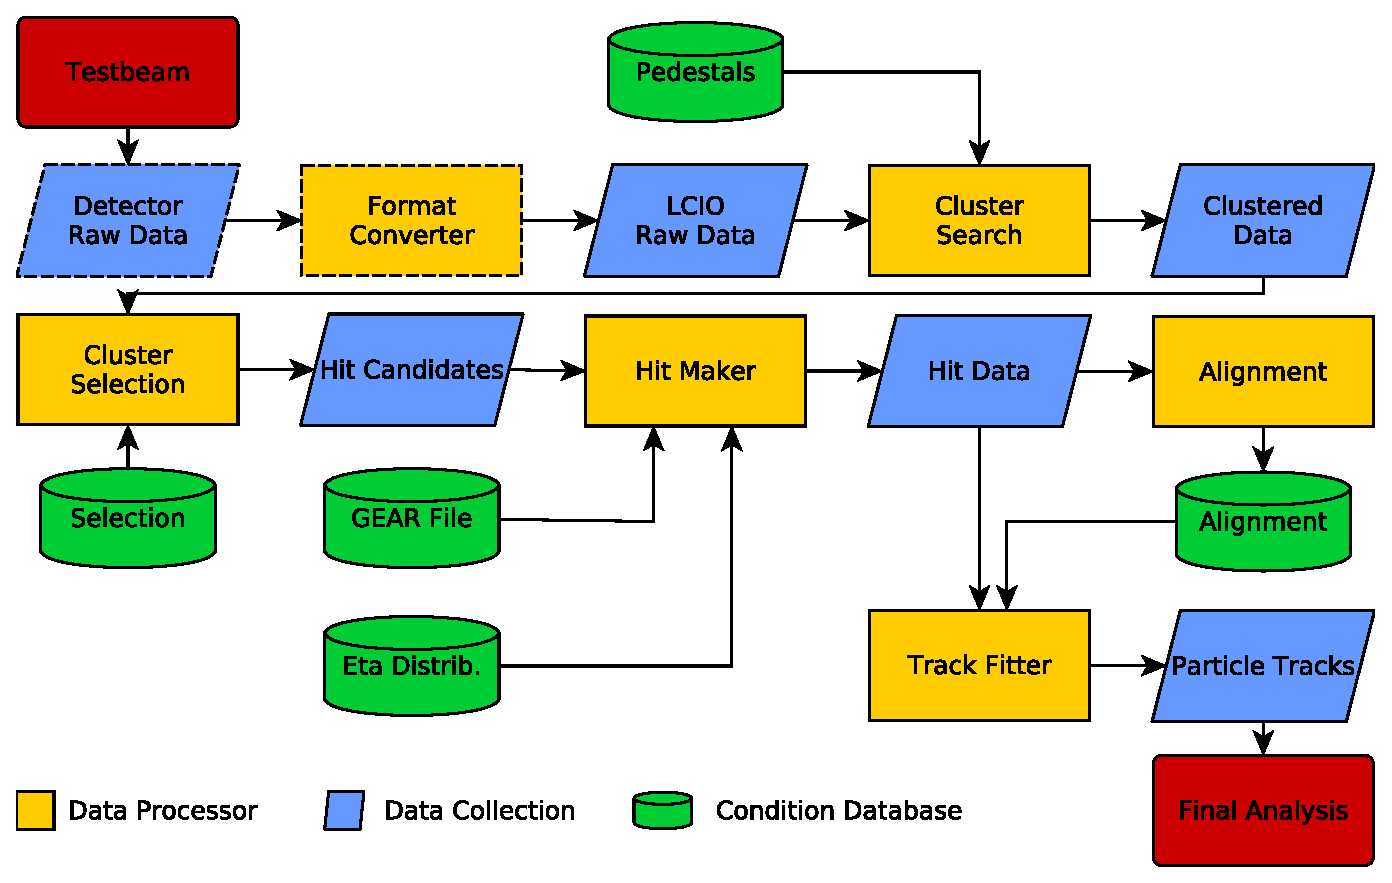
\includegraphics[width=.9\textwidth]{figures/eutel-strategy}
  \caption[The EUTelescope data analysis strategy]{Schematic of the overall telescope data reconstruction and analysis strategy of the EUTelescope framework.
EUTelescope provides processors for all steps, except for the conversion of the DUT raw data, marked with a dashed outline.}
  \label{fig:offline:strategy}
\end{figure}

EUTelescope provides several processors for Marlin, implementing algorithms necessary for a full track reconstruction and data analysis of test beam experiments. 
Figure~\ref{fig:offline:strategy} shows the analysis strategy of the framework starting from the recorded detector response to the final reconstructed particle tracks. 
%An overview of the processor range provided by EUTelescope is given in \cite{EUDET-2007-20}.
At low-energy beam lines such as the DESY-II test beam facility, multiple scattering is an important contribution to the overall track resolution uncertainty,
 especially in measurements with non-negligible DUT material budget, cf.\ section~\ref{sec:multiplescattering}.
Therefore, EUTelescope provides processors implementing advanced algorithms for tracking such as Deterministic Annealing Filter (DAF)~\cite{ref:daffitter}
 or GBL which account for scattering in all material present in the beam.
For high-energy beam lines a simple straight line fit provides sufficient precision and a maximum of computational performance.
In addition, precise offline detector alignment can be performed by minimising track residuals using the EUTelescope alignment processor which utilises the Millepede-II algorithm~\cite{Blobel-2006}.

EUTelescope comes with its own job submission framework Jobsub that allows to run analysis jobs on local machines or to submit them to larger computing clusters such as NAF for bulk reconstruction.
Using its flexible configuration file concept and the global run database storing user defined variables,
 jobsub eases the implementation of per-run variables for reconstruction such as beam energy or detector alignment.

 
The track parameters are calculated by employing a $\chi^{2}$-minimisation method~\cite{ref:eudetmemo_2007_01,ref:lutzpaper}.
For each telescope sensor dimension ($x$ and $y$), the individual contribution $\Delta \chi^2_{i}$ from plane $i$ is defined as

\begin{equation}
\label{eq:chi2contrib}
\Delta \chi^2_{i} = \left( \frac{r - p_{i}}{\sigmai} \right)^2 \Bigg|_{i \ne i_{\textrm{DUT}}} +
\left( \frac{\theta_{\textrm{i}} - \theta_{i-1}}{\Theta_{0}} \right)^2 \Bigg|_{i \ne 0,N-1} \,,
\end{equation}

\noindent
with the telescope plane numbering beginning at zero.
The measured hit position in one dimension is denoted by $r$, the position extrapolated from the track in the same dimension by $p_{i}$.
The angles between the nominal beam direction and the track direction are $\theta_{i-1}$ and $\theta_{i}$.
The former is the track angle entering plane $i$, the latter the angle of the outbound track segment.
The intrinsic resolution of sensor plane $i$ and the width of the multiple scattering distribution are denoted $\sigmai$ and $\Theta_{0}$, respectively, cf.~also section~\ref{sec:multiplescattering}. 
It is assumed that $\sigmai$ and $\Theta_{0}$ do not differ between planes and that $\sigmai$ is also equal for both measurement dimensions.
If the beam axis is denoted by $z$, then $\theta_i$ can be expressed as

\begin{equation}
\theta_i = \frac{p_{i+1} - p_i}{z_{i+1} - z_i} \,.
\end{equation}

\noindent In equation~(\ref{eq:chi2contrib}) the first term, resulting from the hit measurement, is excluded in the $\chi^2$ calculation if the considered plane is the DUT.
Similarly, for the first and last planes the second term in equation~(\ref{eq:chi2contrib}) is omitted, since the scattering angle can not be determined.
This results in the global $\chi^2$ expression

\begin{equation}
\label{eq:globalchi2}
\chi^2 = \sum_{i=0}^{N-1} \alpha_i \left( r - p_i \right)^2 + \sum_{i=1}^{N-2}
\left( \frac{p_{i + 1} \beta_i + p_{i-1} \beta_{i-1} - p_i \left( \beta_i + \beta_{i-1} \right)}{\Theta_0} \right)^2 \,,
\end{equation}

\noindent
with coefficients $\alpha_i$ and $\beta_i$ defined as~\cite{ref:eudetmemo_2007_01}

\begin{equation}
\alpha_i = \left\{
  \begin{array}{l l}
    \sigmai^{-2} & \quad \text{for $i \neq i_{\textrm{DUT}}$}\\
    0 & \quad \text{for $i = i_{\textrm{DUT}}$}
  \end{array} \right. \quad \text{and} \quad \beta_i = \frac{1}{z_{i + 1} - z_i} \,.
\end{equation}

\noindent
which is minimised with respect to the track parameters $p_i$. 
